\section{Recursion}
\label{sec:rec}
This section presents syntax and semantics of probabilistic recursion. We use the Kleene fixed-point theorem to construct fixed points iteratively. 

\subsection{Probabilistic loops}
%Provided that $(L, \leq)$ is a complete lattice and $F: L \fun L$ is monotonic, 
We introduce the syntax for the least fixed point and the greatest fixed point based on the Knaster–Tarski fixed-point theorem~\ref{thm:tarski_fixed_point}. 

\begin{definition}[Least and greatest fixed points]
    \isalink{https://github.com/RandallYe/probabilistic_programming_utp/blob/336ff3c17af12fd71446a50244ff04966bfa71e8/probability/probabilistic_relations/utp_prob_rel_lattice.thy\#L378}
    \begin{align*}
        &\lfp~X @ P \defs \thlfp{}~\left(\lambda X @ P\right)\tag*{(least fixed point)} \label{def:lfp}\\ 
        &\gfp~X @ P \defs \thgfp{}~\left(\lambda X @ P\right)\tag*{(great fixed point)} \label{def:gfp}
    \end{align*}
\end{definition}

We define a loop function $\lfun$ below and use it to define probabilistic while loops later.
\begin{definition}[Loop function]
    We fix a homogeneous relation $b:[S]\hrel$, and homogeneous probabilistic programs $P$ and $X$ of type $[S]\prhfun$, then
    \isalink{https://github.com/RandallYe/probabilistic_programming_utp/blob/336ff3c17af12fd71446a50244ff04966bfa71e8/probability/probabilistic_relations/utp_prob_rel_lattice.thy\#L396}
    \begin{align*}
        &\lfunp{b}{P}{X} \defs~\pcchoice{b}{\left(\pseq{P}{X}\right)}{\pskip} \tag*{(loop function)} \label{def:lfun} 
    \end{align*}
\end{definition}
The function $\lfun$ is a conditional choice between the sequence $\left(\pseq{P}{X}\right)$ and the skip $\pskip$, depending on the relation $b$. We use $\lfunbp$ as a shorthand for $\lambda X @ \lfun(b, P, X)$. The $\lfunbp(X)$ can be simplified. 
%
\begin{align*}
   &\lfunbp(X)\\
 = & \cmt{Definition~\ref{def:lfun} } \\
   & \pcchoice{b}{\left(\pseq{P}{X}\right)}{\pskip} \\
 = & \cmt{Theorem~\ref{thm:prog_cond_choice} Law~\ref{thm:cchoice_pchoice} and Definition~\ref{def:prog_skip}} \\
 & \left(\ppchoice{\rvprfunsym{\ibracket{b}}}{\left(\pseq{P}{X}\right)}{\rvprfunsym{\ibracket{\II}}}\right) \\
 = & \cmt{Theorem~\ref{thm:prob_prob_choice} Law~\ref{thm:pchoice_altdef}} \\
 & \rvprfunsym{\prrvfunsym{\left(\rvprfunsym{\ibracket{b}}\right)}*\prrvfunsym{\left(\pseq{P}{X}\right)} + \left(\rfone - \prrvfunsym{\left(\rvprfunsym{\ibracket{b}}\right)}\right) * \prrvfunsym{\left(\rvprfunsym{\ibracket{\II}}\right)}} \\
 = & \cmt{Theorem~\ref{thm:prrvfun_inverse}, Theorem~\ref{thm:pskip} Law~\ref{thm:pskip_inverse}, Theorem~\ref{thm:prob_assign_finaldist}, and Theorem~\ref{thm:final_distribtion} Law~\ref{thm:final_distribtion_1}} \\
 & \rvprfunsym{{\ibracket{b}}*\prrvfunsym{\left(\pseq{P}{X}\right)} + \left(\rfone - {\ibracket{b}}\right) * {\ibracket{\II}}} \\
 = & \cmt{Theorem~\ref{thm:ib} Law~\ref{thm:ib_neg}} \\
 & \rvprfunsym{{\ibracket{b}}*\prrvfunsym{\left(\pseq{P}{X}\right)} + \ibracket{\lnot b} * {\ibracket{\II}}}\tag*{($lfun$ altdef)} \label{thm:lfun_altdef}
\end{align*}

If a probabilistic program $P$ is a distribution, then $\lfunbp$ is monotonic.
\begin{thm}
    $\isfinaldist\left(\prrvfunsym{P}\right) \implies \mono\left(\lfunbp\right)$
    \isalink{https://github.com/RandallYe/probabilistic_programming_utp/blob/336ff3c17af12fd71446a50244ff04966bfa71e8/probability/probabilistic_relations/utp_prob_rel_lattice_laws.thy\#L4027}
\end{thm}

With $\lfun$, we define two probabilistic loops using both the least and the greatest fixed points. The reason to define two probabilistic loops is our intention to establish the uniqueness theorem of fixed points. Based on Knaster–Tarski fixed-point Theorem~\ref{thm:tarski_fixed_point}, the uniqueness is equivalent to the equality of the least fixed point and the greatest fixed point.

\begin{definition}[Probabilistic loops]
    \isalink{https://github.com/RandallYe/probabilistic_programming_utp/blob/336ff3c17af12fd71446a50244ff04966bfa71e8/probability/probabilistic_relations/utp_prob_rel_lattice.thy\#L399}
    \begin{align*}
%        &\lfp X @ P \defs \thninf{} \left\{u : L | (\lambda X @ P)(u) \leq u\right\} \tag*{(least fixed point)} \label{def:lfp}\\ 
%        &\gfp X @ P \defs \thnsup{} \left\{u : L | u \leq (\lambda X @ P)(u)\right\} \tag*{(great fixed point)} \label{def:gfp}\\
%        &\lfunp{b}{P}{X} \defs \pcchoice{b}{\left(\pseq{P}{X}\right)}{\pskip} \tag*{[Loop body function]} \label{def:lfun}\\
        \pwhile{b}{P} &\defs \lfp~X @ \lfunbp(X) \tag*{(while loop by least fixed point)} \label{def:pwhile}\\
        \pwhiletop{b}{P} &\defs \gfp~X @ \lfunbp(X) \tag*{(while loop by strongest fixed point)} \label{def:pwhile_top}
    \end{align*}
\end{definition}

The $\pwhile{b}{P}$ satisfy several laws below.
\begin{thm}
    \label{thm:pwhile_bot}
    \isalink{https://github.com/RandallYe/probabilistic_programming_utp/blob/336ff3c17af12fd71446a50244ff04966bfa71e8/probability/probabilistic_relations/utp_prob_rel_lattice_laws.thy\#L4160}
\begin{align*}
    & \isfinaldist\left(\prrvfunsym{P}\right) \implies \pwhile{b}{P} = \lfunbp\left(\pwhile{b}{P}\right) \tag*{(unfold)} \label{thm:pwhile_unfold}\\
    & \pwhile{\ufalse}{P} = \pskip \tag*{(false)} \label{thm:pwhile_false}\\
    & \pwhile{\utrue}{P} = \ufzero \tag*{(true)} \label{thm:pwhile_true}
\end{align*}
\end{thm}
If $P$ is a distribution, $\pwhile{b}{P}$ can be unfolded without its semantics changed. If $b$ is $\ufalse$, the loop is just $\pskip$. It is $\ufzero$ otherwise.

The $\pwhiletop{b}{P}$ satisfy similar laws below.
\begin{thm}
    \label{thm:pwhile_top}
    \isalink{https://github.com/RandallYe/probabilistic_programming_utp/blob/336ff3c17af12fd71446a50244ff04966bfa71e8/probability/probabilistic_relations/utp_prob_rel_lattice_laws.thy\#L4197}
\begin{align*}
    \isfinaldist\left(\prrvfunsym{P}\right) \implies & \pwhiletop{b}{P} = \lfunbp\left(\pwhiletop{b}{P}\right) \tag*{(unfold)} \label{thm:pwhiletop_unfold}\\
    & \pwhiletop{\ufalse}{P} = \pskip \tag*{(false)} \label{thm:pwhiletop_false}\\
    \isfinaldist\left(\prrvfunsym{P}\right) \implies & \pwhiletop{\utrue}{P} = \ufone \tag*{(true)} \label{thm:pwhiletop_true}
\end{align*}
\end{thm}
We note that if $P$ is a distribution and $b$ is $\utrue$, the loop is just $\ufone$, instead of $\ufzero$ for $\pwhileop$. 

As the semantics for probabilistic loops in our programming language is the \ref{def:tarski_lfp} and the \ref{def:tarski_gfp} in Knaster–Tarski fixed-point Theorem~\ref{thm:tarski_fixed_point}, this does not give information about how fixed points can be computed by iterations. We resort to Kleene fixed-point Theorem~\ref{thm:kleene_fixed_point_theorem} for iterations. Our use of iterations to compute fixed point is motivated by a simple probabilistic program: flip a coin until the outcome is a head, defined as follows.

\subsection{Motivation example}
This example~\cite{Kozen1985,Morgan1996,Dahlqvist2020} is about flipping a coin till the outcome is a head. 
\begin{definition}[Flip a coin]
    \label{def:coin_flip}
    \isalink{https://github.com/RandallYe/probabilistic_programming_utp/blob/336ff3c17af12fd71446a50244ff04966bfa71e8/probability/probabilistic_relations/Examples/utp_prob_rel_lattice_coin.thy\#L14}
    \begin{align*}
        & Tcoin ::= hd | tl \\ 
        & \isakwmaj{alphabet}\ cstate = c::Tcoin \\
        & cflip \defs \ppchoice{1/2}{\passign{c}{hd}}{\passign{c}{tl}} \\
        & flip \defs \pwhile{c = tl}{cflip}
    \end{align*}
\end{definition}
$Tcoin$ is a free type in the Z notation or an enumerable data type in Isabelle, and it contains two constants $hd$ and $tl$ of type $Tcoin$. The keyword $\isakwmaj{alphabet}$ is used to declare the state space of a program and it is $cstate$ in this case. This state space is composed of only one variable $c$ of type $Tcoin$, denoting the outcome of the coin flip experiment. The $cflip$ is a probabilistic choice denoting both $hd$ and $tl$ are equally likely, or a uniform distribution over two outcomes. Finally, this program $flip$ is a while loop whose condition is $c = tl$, specifying that the outcome is $tl$, and whose body is $cflip$.
%
The $cflip$ is simplified as follows.
\begin{align*}
   &cflip \\
 = & \cmt{Definition of $cflip$ } \\
   & \ppchoice{1/2}{\passign{c}{hd}}{\passign{c}{tl}}  \\
 = & \cmt{Law~\ref{thm:pchoice_altdef} in Theorem~\ref{thm:prob_prob_choice} and Definition~\ref{def:prog_assign}} \\
 & \rvprfunsym{\prrvfunsym{1/2}*\prrvfunsym{\left(\rvprfunsym{\ibracket{\passign{c}{hd}}}\right)} + \left(\rfone - \prrvfunsym{1/2}\right) * \prrvfunsym{\left(\rvprfunsym{\ibracket{\passign{c}{tl}}}\right)}} \\
 = & \cmt{Conversion Definitions~\ref{def:rvfun2prfun} and~\ref{def:u2r_r2u}, and Theorem~\ref{thm:prrvfun_inverse}} \\
 & \rvprfunsym{{1/2}*{\ibracket{\passign{c}{hd}}} + {1/2} * {\ibracket{\passign{c}{tl}}}} \\
 = & \cmt{Definition~\ref{def:uassign}} \\
 & \rvprfunsym{{1/2}*{\ibracket{c' = hd}} + {1/2} * {\ibracket{c' = tl}}} \tag*{($cflip$ altdef)} \label{thm:cflip_altdef}
\end{align*}
The $cflip$ is also a distribution.
\begin{lem}
    \label{thm:cflip_distribution}
    $\isfinaldist(\prrvfunsym{cflip})$ 
    \isalink{https://github.com/RandallYe/probabilistic_programming_utp/blob/336ff3c17af12fd71446a50244ff04966bfa71e8/probability/probabilistic_relations/Examples/utp_prob_rel_lattice_coin.thy\#L39}
\end{lem}
\begin{proof}
   \begin{align*}
    & \cmt{Theorem~\ref{thm:prob_assign_finaldist}} \\
    & \isfinaldist(\prrvfunsym{\passign{c}{hd}})  \land  \isfinaldist(\prrvfunsym{\passign{c}{tl}}) \\
    \implies & \cmt{Theorem~\ref{thm:prob_prob_choice} Law~\ref{thm:pchoice_final_dist}} \\
    & \isfinaldist(\prrvfunsym{cflip}) 
   \end{align*}
\end{proof}

Then the loop function $\lfun_{cflip}^{c = tl}(X)$, denoted as $\lfun_c$, is further simplified.
\begin{align*}
   & \lfun_c(X) \\
 = & \cmt{Law~\ref{thm:lfun_altdef}} \\
 & \rvprfunsym{{\ibracket{c=tl}}*\prrvfunsym{\left(\pseq{cflip}{X}\right)} + {\ibracket{\lnot c=tl}} * {\ibracket{\II}}} \\ 
 = & \cmt{Law~\ref{thm:cflip_altdef}, Theorem~\ref{def:utp_relation} Law~\ref{def:uskip}, and Thoerem~\ref{thm:ib} Law~\ref{thm:ib_conj}} \\
 & \rvprfunsym{{\ibracket{c=tl}}*\prrvfunsym{\left(\pseq{\left(\rvprfunsym{{1/2}*{\ibracket{c' = hd}} + {1/2} * {\ibracket{c' = tl}}} \right)}{X}\right)} + {\ibracket{\lnot c=tl}*\ibracket{c'=c}}} \\ 
 = & \cmt{Definition~\ref{def:coin_flip} of $Tcoin$: $(\lnot c = tl) = (c = hd)$} \\
 & \rvprfunsym{{\ibracket{c=tl}}*\prrvfunsym{\left(\pseq{\left(\rvprfunsym{{1/2}*{\ibracket{c' = hd}} + {1/2} * {\ibracket{c' = tl}}} \right)}{X}\right)} + {\ibracket{c=hd}*\ibracket{c'=c}}} \tag*{(loop body of $flip$)} \label{thm:F_cflip_tl_altdef} 
\end{align*}
Now consider $F^n(\bot)$ in the Kleene fixed-point theorem, and here $F$ is $\lfun_c$ and $\bot$ is $\ufzero$.
\begin{align*}
\left(\lfun_c\right)^0(\ufzero) =& \ufzero \\
%
\left(\lfun_c\right)^1(\ufzero) 
 =&\cmt{Law~\ref{thm:F_cflip_tl_altdef}} \\
& \rvprfunsym{{\ibracket{c=tl}}*\prrvfunsym{\left(\pseq{\left(\rvprfunsym{{1/2}*{\ibracket{c' = hd}} + {1/2} * {\ibracket{c' = tl}}} \right)}{\ufzero}\right)} + {\ibracket{c=hd}*\ibracket{c'=c}}}\\
 =&\cmt{Right Zero Theorem~\ref{thm:prog_seq_comp} Law~\ref{thm:pseq_right_zero}} \\
 & \rvprfunsym{{\ibracket{c=hd}*\ibracket{c'=c}}} \\
%
\left(\lfun_c\right)^2 (\ufzero) 
 = &\cmt{$F^2(\ufzero) = F(F^1(\ufzero))$ and Law~\ref{thm:lfun_altdef}} \\
 & \rvprfunsym{{\ibracket{c=tl}}*\prrvfunsym{\left(\pseq{cflip}{\left(F_{cflip}^{c=tl}\right)^1(\ufzero) }\right)} + {\ibracket{\lnot c=tl}} * {\ibracket{\II}}} \\ 
 = & \cmt{Law~\ref{thm:cflip_altdef}, ${\left(F_{cflip}^{c=tl}\right)^1(\ufzero)}$, Theorem~\ref{def:utp_relation} Law~\ref{def:uskip}, and Thoerem~\ref{thm:ib} Law~\ref{thm:ib_conj}} \\
 & \rvprfunsym{{\ibracket{c=tl}}*\prrvfunsym{\left(\pseq{\left(\rvprfunsym{{1/2}*{\ibracket{c' = hd}} + {1/2} * {\ibracket{c' = tl}}} \right)}{\rvprfunsym{{\ibracket{c=hd}*\ibracket{c'=c}}}}\right)} + {\ibracket{c=hd}*\ibracket{c'=c}}} \\ 
 = & \cmt{Definition~\ref{def:prog_seq}, Thoerem~\ref{thm:ib}, Theorem~\ref{thm:pseq_ibracket_contradictory}, $\cdots$} \\
 & \rvprfunsym{{\ibracket{c=tl}}*{\ibracket{c' = hd}}/2 + {\ibracket{c=hd}*\ibracket{c'=c}}} \\ 
	%
\left(\lfun_c\right)^3 (\ufzero)
 = & \cmt{$\cdots$} \\
 & \rvprfunsym{{\ibracket{c=tl}}*{\ibracket{c' = hd}}/2 + {\ibracket{c=tl}}*{\ibracket{c' = hd}}/2^2 + {\ibracket{c=hd}*\ibracket{c'=c}}} \\ 
 = & \cmt{$\cdots$} \\
 & \rvprfunsym{{\ibracket{c=tl}}*{\ibracket{c' = hd}}*\left(1/2 + 1/2^2\right) + {\ibracket{c=hd}*\ibracket{c'=c}}} \\ 
		%
 & \cdots \\
\left(\lfun_c\right)^n (\ufzero) 
 = & \cmt{Induction} \\
 & \rvprfunsym{{\ibracket{c=tl}}*{\ibracket{c' = hd}}*\left(1/2 + 1/2^2 + \cdots + 1/2^{(n-1)}\right) + {\ibracket{c=hd}*\ibracket{c'=c}}} \\ 
 = & \cmt{Summation} \\
 & \rvprfunsym{{\ibracket{c=tl}}*{\ibracket{c' = hd}}* \sum_{i=1}^{n-1} 1/2^{i} + {\ibracket{c=hd}*\ibracket{c'=c}}} \tag*{(iteration from bot)} \label{thm:F_b_P_clip_bot} 
%
\end{align*}
%
The $\left(\lfun_c\right)^n (\ufzero)$ corresponds to the termination probability after up to $n-1$ iterations of the loop body of $flip$ in Definition~\ref{def:coin_flip}. For example, $\left(\lfun_c\right)^1 (\ufzero)$ corresponds to zero iterations or immediate termination . Its semantics is $\rvprfunsym{{\ibracket{c=hd}*\ibracket{c'=c}}}$ which means if the initial value of $c$ is $hd$, then the final value is also $hd$ with probability 1. 
%It terminates only if the initial value of $c$ is $hd$. 
For example, $\left(\lfun_c\right)^3 (\ufzero)$ corresponds to the termination after up to two iterations including the immediate termination, the termination after exact one iteration (${\ibracket{c=tl}}*{\ibracket{c' = hd}}/2$, meaning the initial value of $c$ is $tl$ and the outcome of the flip is $hd$ with probability $1/2$), and exact two iterations (${\ibracket{c=tl}}*{\ibracket{c' = hd}}/2^2$).  

Now consider $F^n(\top)$ in the Kleene fixed-point theorem, and here $\top$ is $\ufone$.
\begin{align*}
\left(\lfun_c\right)^0(\ufone) =& \ufone\\
%
\left(\lfun_c\right)^1(\ufone) 
 =&\cmt{Law~\ref{thm:F_cflip_tl_altdef}} \\
& \rvprfunsym{{\ibracket{c=tl}}*\prrvfunsym{\left(\pseq{\left(\rvprfunsym{{1/2}*{\ibracket{c' = hd}} + {1/2} * {\ibracket{c' = tl}}} \right)}{\ufone}\right)} + {\ibracket{c=hd}*\ibracket{c'=c}}}\\
 =&\cmt{Lemma~\ref{thm:cflip_distribution} and Theorem~\ref{thm:prog_seq_comp} Law~\ref{thm:pseq_one}} \\
 & \rvprfunsym{{\ibracket{c=tl}} + {\ibracket{c=hd}*\ibracket{c'=c}}} \\
%
\left(\lfun_c\right)^2 (\ufone) 
 = &\cmt{$F^2(\ufone) = F(F^1(\ufone))$ and Law~\ref{thm:lfun_altdef}} \\
 & \rvprfunsym{{\ibracket{c=tl}}*\prrvfunsym{\left(\pseq{cflip}{\left(F_{cflip}^{c=tl}\right)^1(\ufone) }\right)} + {\ibracket{\lnot c=tl}} * {\ibracket{\II}}} \\ 
 = & \cmt{Law~\ref{thm:cflip_altdef}, ${\left(F_{cflip}^{c=tl}\right)^1(\ufone)}$, Theorem~\ref{def:utp_relation} Law~\ref{def:uskip}, and Thoerem~\ref{thm:ib} Law~\ref{thm:ib_conj}} \\
 & \rvprfunsym{{\ibracket{c=tl}}*\prrvfunsym{\left(\pseq{\left(\rvprfunsym{
     \begin{array}[]{l}
     {1/2}*{\ibracket{c' = hd}} + \\
     {1/2} * {\ibracket{c' = tl}}
     \end{array}
 } \right)}{\left(\rvprfunsym{
     \begin{array}[]{l}
        {\ibracket{c=tl}} + \\
        {\ibracket{c=hd}*\ibracket{c'=c}}
     \end{array}
 }\right)}\right)} + {\ibracket{c=hd}*\ibracket{c'=c}}} \\ 
 = & \cmt{Definition~\ref{def:prog_seq}, Thoerems~\ref{thm:ib}, Theorem~\ref{thm:pseq_ibracket_contradictory}, $\cdots$} \\
 & \rvprfunsym{{\ibracket{c=tl}}*\prrvfunsym{\left({\rvprfunsym{
     \begin{array}[]{l}
     {1/2} * {\ibracket{c' = hd}} + {1/2}
     \end{array}
 } }\right)} + {\ibracket{c=hd}*\ibracket{c'=c}}} \\ 
 = & \cmt{ Theorem~\ref{thm:prrvfun_inverse} } \\
 & \rvprfunsym{{\ibracket{c=tl}/2}+ {\ibracket{c=tl}} * {\ibracket{c' = hd}}/2 + {\ibracket{c=hd}*\ibracket{c'=c}}} \\ 
	%
\left(\lfun_c\right)^3 (\ufone)
 = & \cmt{$\cdots$} \\
 & \rvprfunsym{{\ibracket{c=tl}/2^2} + {\ibracket{c=tl}}*{\ibracket{c' = hd}}*\left(1/2 + 1/2^2\right) + {\ibracket{c=hd}*\ibracket{c'=c}}} \\ 
		%
 & \cdots \\
\left(\lfun_c\right)^n (\ufone) 
 = & \cmt{Induction} \\
 & \rvprfunsym{{\ibracket{c=tl}/2^{n-1}} + {\ibracket{c=tl}}*{\ibracket{c' = hd}}* \sum_{i=1}^{n-1} 1/2^{i} + {\ibracket{c=hd}*\ibracket{c'=c}}} \tag*{(iteration from top)} \label{thm:F_b_P_clip_top} 
%
\end{align*}
We notice that $\left(\lfun_c\right)^n (\ufone)$ above is an addition of three operands of which the last two are the same as $\left(\lfun_c\right)^n (\ufzero)$ in \ref{thm:F_b_P_clip_bot}. The extra operand ${\ibracket{c=tl}/2^{n-1}}$ converges to 0 when $n$ approaches $\infty$, and so eventually $\left(\lfun_c\right)^n (\ufzero)$ and $\left(\lfun_c\right)^n (\ufone)$ coincide at $\infty$. This is illustrates in Fig.~\ref{fig:coin_t_prob_iteration} where the common part ${\ibracket{c=hd}*\ibracket{c'=c}}$ in $\left(\lfun_c\right)^n (\ufzero)$ and $\left(\lfun_c\right)^n (\ufone)$ is omitted.
%
\begin{figure}[!ht]
    \begin{center}
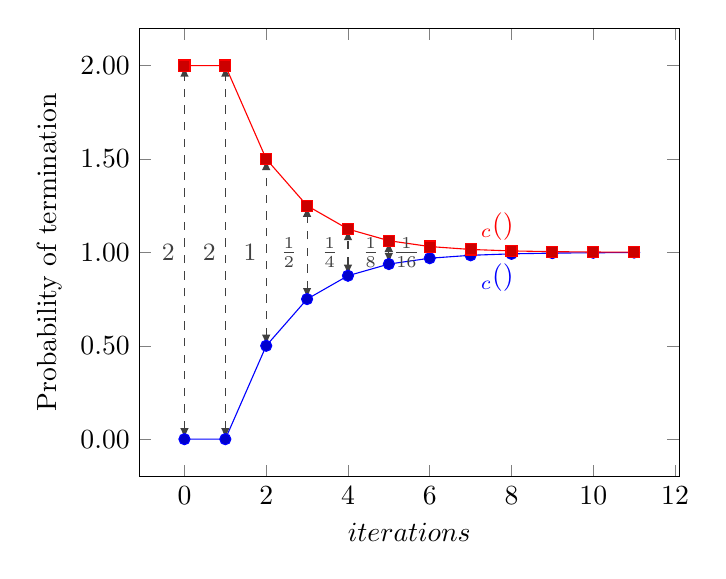
\begin{tikzpicture}
\begin{axis}[%[ybar] 
    xlabel={$iterations$},
    ylabel={Probability of termination},
    y tick label style={/pgf/number format/.cd,fixed,fixed zerofill,precision=2},
]
    \addplot table[header=false,col sep=&,row sep=\\,y expr={\thisrowno{1}}] {
        0 & 0\\
        1 & 0\\
        2 & 1 - 1/2^1\\
        3 & 1 - 1/2^2\\
        4 & 1 - 1/2^3\\
        5 & 1 - 1/2^4\\
        6 & 1 - 1/2^5\\
        7 & 1 - 1/2^6\\
        8 & 1 - 1/2^7\\
        9 & 1 - 1/2^8\\
        10& 1 - 1/2^9\\
        11& 1 - 1/2^10\\
        %12& 1 - 1/2^11\\
        %13& 1 - 1/2^12\\
        %14& 1 - 1/2^13\\
        %15& 1 - 1/2^14\\
    } node[below,pos=0.7] {$\lfun_c(\ufzero)$};

    \addplot table[header=false,col sep=&,row sep=\\,y expr={\thisrowno{1}}] {
        0 & 2\\
        1 & 2\\
        2 & 2/2^1 + 1 - 1/2^1 \\
        3 & 2/2^2  + 1 - 1/2^2 \\
        4 & 2/2^3  + 1 - 1/2^3 \\
        5 & 2/2^4  + 1 - 1/2^4 \\
        6 & 2/2^5  + 1 - 1/2^5 \\
        7 & 2/2^6  + 1 - 1/2^6 \\
        8 & 2/2^7  + 1 - 1/2^7 \\
        9 & 2/2^8  + 1 - 1/2^8 \\
        10& 2/2^9  + 1 - 1/2^9 \\
        11& 2/2^10 + 1 - 1/2^10\\
        %12& 2/2^11 + 1 - 1/2^11\\
        %13& 2/2^12 + 1 - 1/2^12\\
        %14& 2/2^13 + 1 - 1/2^13\\
        %15& 2/2^14 + 1 - 1/2^14\\
    } node[above,pos=0.7] {$\lfun_c(\ufone)$};

    % \draw (axis cs:1,0) -- node[left]{Text} (axis cs:1,2);
    \draw[latex-latex, darkgray, dashed] (axis cs:0,0) -- node[left]{\small 2} (axis cs:0,2);
    \draw[latex-latex, darkgray, dashed] (axis cs:1,0) -- node[left]{\small 2} (axis cs:1,2);
    \draw[latex-latex, darkgray, dashed] (axis cs:2, 1 - 1/2^1) -- node[left]{\small 1} (axis cs:2, 2/2^1 + 1 - 1/2^1);
    \draw[latex-latex, darkgray, dashed] (axis cs:3, 1 - 1/2^2) -- node[left]{\small $\frac{1}{2}$} (axis cs:3, 2/2^2 + 1 - 1/2^2);
    \draw[latex-latex, darkgray, dashed] (axis cs:4, 1 - 1/2^3) -- node[left]{\small $\frac{1}{4}$} (axis cs:4, 2/2^3 + 1 - 1/2^3);
    \draw[latex-latex, darkgray, dashed] (axis cs:5, 1 - 1/2^4) -- node[left]{\small $\frac{1}{8}$} (axis cs:5, 2/2^4 + 1 - 1/2^4);
    \draw[latex-latex, darkgray, dashed] (axis cs:6, 1 - 1/2^5) -- node[left]{\small $\frac{1}{16}$} (axis cs:6, 2/2^5 + 1 - 1/2^5);
    %\draw[latex-latex, darkgray, dashed] (axis cs:7, 1 - 1/2^6) -- (axis cs:7, 2/2^6 + 1 - 1/2^6);
    % \addplot[mark=*, red, dashed] table[header=false,col sep=&,row sep=\\,y expr={\thisrowno{1}}] {
%        0 & 0\\
%        0 & 2\\
%    };
  \end{axis}
\end{tikzpicture}
    \end{center}
    \caption{Termination probability over iterations from bottom and top for coin flip.}
    \label{fig:coin_t_prob_iteration}
\end{figure}
%
As shown in the diagram, along with the increasing iterations, $\left(\lfun_c\right)^n (\ufzero)$ increases towards 1 from the initial 0, while $\left(\lfun_c\right)^n (\ufone)$ decreases towards 1 from the initial 2. Their differences, marked with dashed lines, are becoming smaller and smaller.
From this example, we observe that there is one unique fixed point where the least fixed point and the greatest fixed point are the same. The precondition for this uniqueness is their iteration differences converging to 0. If this is the case, in order to reason about a probabilistic loop, we just need to find out a fixed point and prove it. Then the fixed point is the semantics of the loop. Actually, we do not need to compute it by iterations. 

This example motivates us to give a semantics to probabilistic loops as follows.
First, we need to prove the loop function is continuous. Then if the differences of iterations from top and bottom converges to 0, there is a unique fixed point. Otherwise, we use the Kleene fixed-point Theorem~\ref{thm:kleene_fixed_point_theorem} to compute the least fixed point and the greatest fixed point by iterations.

\subsection{Fixed point theorems}
We define the function $\iter$ below recursively for iterations $(\lfun_P^b)^n(X)$, and the function $\iterdiff$ for the differences between iterations from top and bottom.
\begin{definition}[Iteration and iteration difference]
    \isalink{https://github.com/RandallYe/probabilistic_programming_utp/blob/336ff3c17af12fd71446a50244ff04966bfa71e8/probability/probabilistic_relations/utp_prob_rel_lattice.thy\#L405}
    \begin{align*}
        &\iter\left(n, b, P, X\right) \defs \left(\IF n = 0 \THEN X \ELSE \lfunbp\left(\iter\left(n-1, b, P, X\right)\right)\right)\tag*{(iteration)} \label{def:iter}\\
        &\lfundiff(b,P,X) \defs~\pcchoice{b}{\left(\pseq{P}{X}\right)}{\clz \ufzero} \\%\tag*{(loop function bottom)} \label{def:lfundiff} \\ 
        % &\iterdiff\left(n, b, P, X\right) \defs \left(\IF n = 0 \THEN X \ELSE \left(\pcchoice{b}{\left(\pseq{P}{\iterdiff\left(n-1, b, P, X\right)}\right)}{\ufzero}\right)\right)\tag*{(iteration difference)} \label{def:iterdiff}
        &\iterdiff\left(n, b, P, X\right) \defs \left(\IF n = 0 \THEN X \ELSE \lfundiff\left(b, P, \iterdiff\left(n-1, b, P, X\right)\right)\right)\tag*{(iteration difference)} \label{def:iterdiff}
    \end{align*}
\end{definition}
The $\lfundiff$ is similar to $\lfun$ in Definition~\ref{def:lfun} except that if the condition $b$ does not hold, it is $\ufzero$ instead of $\pskip$ in $\lfun$.

We show that the iteration from bottom is an ascending chain and the iteration from top is a descending chain if $P$ is a distribution.
\begin{thm}%[Iteration from bottom is an ascending chain]
    \label{thm:iter_bot_ascending}
   $\isfinaldist\left(\prrvfunsym{P}\right) \implies \incseq\left(\lambda n @ \iter\left(n, b, P, \ufzero\right)\right)$ 
   \isalink{https://github.com/RandallYe/probabilistic_programming_utp/blob/336ff3c17af12fd71446a50244ff04966bfa71e8/probability/probabilistic_relations/utp_prob_rel_lattice_laws.thy\#L4291}
\end{thm}

\begin{thm}%[Iteration from top is a descending chain]
    \label{thm:iter_top_descending}
   $\isfinaldist\left(\prrvfunsym{P}\right) \implies \decseq\left(\lambda n @ \iter\left(n, b, P, \ufone\right)\right)$ 
   \isalink{https://github.com/RandallYe/probabilistic_programming_utp/blob/336ff3c17af12fd71446a50244ff04966bfa71e8/probability/probabilistic_relations/utp_prob_rel_lattice_laws.thy\#L4331}
\end{thm}

For an ascending or descending chain $f$, we define $\finstatesasc$ and $\finstatesdes$ to denote there are only finite states to have their suprema or infima different from their initial values $f(0)$.
\begin{definition}[Finite states]
    \label{def:finstates}
    We fix $f: \nat \fun [S]\prhfun$, then define
    \isalink{https://github.com/RandallYe/probabilistic_programming_utp/blob/5558d7350b75fd5c1914dd8618d95bfad9e2f789/probability/probabilistic_relations/utp_prob_rel_lattice.thy\#L395}
    \begin{align*}
        \finstatesasc(f) & \defs \finite\left(\left\{s : S \mid \left(\left(\thnsup n @ f(n,s)\right) > f(0,s) \right)\right\}\right) \\
        \finstatesdes(f) & \defs \finite\left(\left\{s : S \mid \left(\left(\thninf n @ f(n,s)\right) < f(0,s) \right)\right\}\right)
    \end{align*}
\end{definition}
The intuition behind the definitions of $\finstatesasc$ and $\finstatesdes$ is that if an ascending or descending chain $f$ has its supremum or infimum not equal to $f(0)$ for a particular state $s$, then there exists a $m:\nat$ such that for any $\varepsilon:\real > 0$, $\left(\thnsup n @ f(n,s) - f(m,s) < \varepsilon\right)$ or $\left(f(m,s) - \thninf n @ f(n,s)  < \varepsilon\right)$. 
%$f(m, s) = f(0, s)$ and $f(m+1, s) > f(m, s)$ or $f(m+1, s) < f(m, s)$.
%
% \begin{definition}[Finite final states]
% %   $finite(P) = \finite\left(\left\{s : S | P(s)\right\}\right)$
% %   $fin\_states(P) = finite\left(\lambda s : S \times S @ \exists n @ \iter\left(n, b, P, \ufzero\right)\right)$
%     \begin{align*}
%         \finstates(f) & \defs \finite\left(\left\{s : S | \left(\left(\thnsup n @ f(n,s)\right) > f(0,s) \right)\right\}\right) \\
%         \finstatesnzero(b, P) & \defs \finite\left(\left\{s : S \times S | \left(\exists n @ \iter\left(n, b, P, \ufzero\right) s \neq 0 \right)\right\}\right) \\
%         \finstatesnone(b, P) & \defs \finite\left(\left\{s : S \times S | \left(\exists n @ \iter\left(n, b, P, \ufone\right) s \neq 1 \right)\right\}\right)
%     \end{align*}
% \end{definition}

We show that if $f$ is an ascending chain and also $\finstatesasc(f)$, then there exists a $N:\nat$ such that for any $n\geq N$, $f(n,s)$ is close to its supremum in a given distance $\varepsilon : \real > 0$ for any $s$. 
\begin{thm}
    \label{thm:incseq_limit_is_lub_all}
    We fix $f:\nat \fun [S_1,S_2]\prfun$, then 
    \isalink{https://github.com/RandallYe/probabilistic_programming_utp/blob/5558d7350b75fd5c1914dd8618d95bfad9e2f789/probability/probabilistic_relations/utp_prob_rel_lattice_laws.thy\#L3487}
    \begin{align*}
        & \incseq(f) \land \finstatesasc(f) \implies \forall \varepsilon:\real > 0 \bullet \exists N:\nat \bullet \forall n \geq N \bullet \forall s \bullet \left(\thnsup m @ f(m, s)\right) - f(n,s) < \varepsilon %\\
%        & \decseq(f) \land \finstatesdes(f) \implies \forall \varepsilon:\real > 0 \bullet \exists N:\nat \bullet \forall n \geq N \bullet \forall s \bullet f(n,s) - \left(\thnsup m @ f(m, s)\right) < \varepsilon
    \end{align*}
\end{thm}

\begin{figure}[!ht]
    \begin{center}
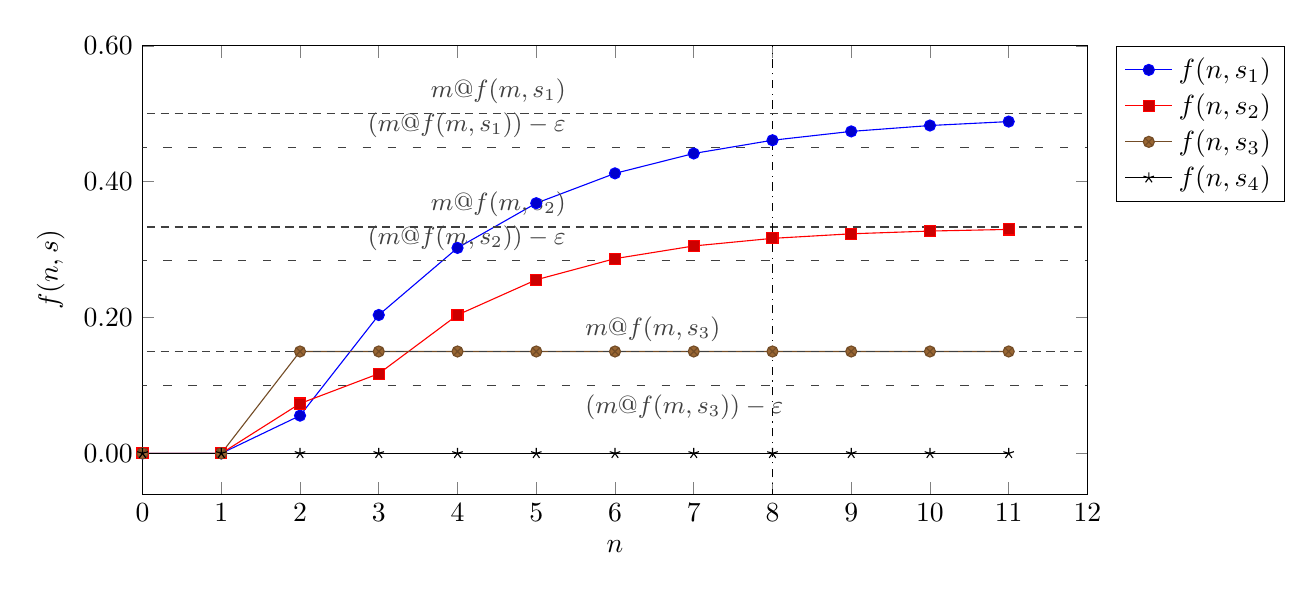
\begin{tikzpicture}
\begin{axis}[%[ybar] 
    xlabel={$n$},
    xmin=0,
    xmax=12,
    x=1.0cm,
    ymax=0.6,
    ylabel={$f(n,s)$},
    y tick label style={/pgf/number format/.cd,fixed,fixed zerofill,precision=2},
    legend pos=outer north east,
]
    \addplot table[header=false,col sep=&,row sep=\\,y expr={\thisrowno{1}}] {
        0 & 0\\
        1 & 0\\
        2 & 1/2 - (2/3)^2\\
        3 & 1/2 - (2/3)^3\\
        4 & 1/2 - (2/3)^4\\
        5 & 1/2 - (2/3)^5\\
        6 & 1/2 - (2/3)^6\\
        7 & 1/2 - (2/3)^7\\
        8 & 1/2 - (2/3)^8\\
        9 & 1/2 - (2/3)^9\\
        10& 1/2 - (2/3)^10\\
        11& 1/2 - (2/3)^11\\
        %12& 1 - 1/2^11\\
        %13& 1 - 1/2^12\\
        %14& 1 - 1/2^13\\
        %15& 1 - 1/2^14\\
    } node[below right,pos=0.7] {};
    \addlegendentry{$f(n,s_1)$};

    \addplot table[header=false,col sep=&,row sep=\\,y expr={\thisrowno{1}}] {
        0 & 0\\
        1 & 0\\
        2 & 1/3 - (3/5)^2 + 0.1\\
        3 & 1/3 - (3/5)^3\\
        4 & 1/3 - (3/5)^4\\
        5 & 1/3 - (3/5)^5\\
        6 & 1/3 - (3/5)^6\\
        7 & 1/3 - (3/5)^7\\
        8 & 1/3 - (3/5)^8\\
        9 & 1/3 - (3/5)^9\\
        10& 1/3 - (3/5)^10\\
        11& 1/3 - (3/5)^11\\
        %12& 1 - 1/2^11\\
        %13& 1 - 1/2^12\\
        %14& 1 - 1/2^13\\
        %15& 1 - 1/2^14\\
    } node[below right,pos=0.7] {};
    % \draw (axis cs:1,0) -- node[left]{Text} (axis cs:1,2);
    \addlegendentry{$f(n,s_2)$};

    \addplot table[header=false,col sep=&,row sep=\\,y expr={\thisrowno{1}}] {
        0 & 0\\
        1 & 0\\
        2 & 0.15\\
        3 & 0.15\\
        4 & 0.15\\
        5 & 0.15\\
        6 & 0.15\\
        7 & 0.15\\
        8 & 0.15\\
        9 & 0.15\\
        10& 0.15\\
        11& 0.15\\
        %12& 1 - 1/2^11\\
        %13& 1 - 1/2^12\\
        %14& 1 - 1/2^13\\
        %15& 1 - 1/2^14\\
    } node[below right,pos=0.7] {};
    \addlegendentry{$f(n,s_3)$};

    \addplot table[header=false,col sep=&,row sep=\\,y expr={\thisrowno{1}}] {
        0 & 0\\
        1 & 0\\
        2 & 0\\
        3 & 0\\
        4 & 0\\
        5 & 0\\
        6 & 0\\
        7 & 0\\
        8 & 0\\
        9 & 0\\
        10& 0\\
        11& 0\\
        %12& 1 - 1/2^11\\
        %13& 1 - 1/2^12\\
        %14& 1 - 1/2^13\\
        %15& 1 - 1/2^14\\
    } node[above right,pos=0.7] {};
    \addlegendentry{$f(n,s_4)$};

    % \draw[darkgray] (axis cs:-1,0.5) -- (axis cs:12,0.5);
    % \node[black,right] at (axis cs:12,0.5){\small $\thnsup m @ f(m,s_1)$};
    % %\draw[darkgray,dashed] (axis cs:-1,0.45) -- node[above right]{\small $\left(\thnsup m @ f(m,s_1)\right) - \varepsilon$} (axis cs:12,0.45);
    % \draw[darkgray,dashed] (axis cs:-1,0.45) -- (axis cs:12,0.45);
    % \node[black,right] at (axis cs:12,0.45){\small $\left(\thnsup m @ f(m,s_1)\right) - \varepsilon$};
    \draw[darkgray,densely dashed] (axis cs:-1,0.5) -- node[above left]{\small $\thnsup m @ f(m,s_1)$} (axis cs:12,0.5);
    \draw[darkgray,loosely dashed] (axis cs:-1,0.45) -- node[above left]{\small $\left(\thnsup m @ f(m,s_1)\right) - \varepsilon$} (axis cs:12,0.45);

    \draw[darkgray,densely dashed] (axis cs:-1,1/3) -- node[above left]{\small $\thnsup m @ f(m,s_2)$} (axis cs:12,1/3);
    \draw[darkgray,loosely dashed] (axis cs:-1,1/3-0.05) -- node[above left]{\small $\left(\thnsup m @ f(m,s_2)\right) - \varepsilon$} (axis cs:12,1/3-0.05);

    \draw[darkgray,densely dashed] (axis cs:-1,0.15) -- node[above right]{\small $\thnsup m @ f(m,s_3)$} (axis cs:12,0.15);
    \draw[darkgray,loosely dashed] (axis cs:-1,0.1) -- node[below right]{\small $\left(\thnsup m @ f(m,s_3)\right) - \varepsilon$} (axis cs:12,0.1);

    \draw[black,dashdotted] (axis cs:8,-1) -- node[above left]{\small $N$} (axis cs:8,0.6);
  \end{axis}
\end{tikzpicture}
    \end{center}
    \caption{Illustration of limits of a increasing chain for various states.}
    \label{fig:finitestateasc}
\end{figure}
%

This is explained and illustrated in Fig.~\ref{fig:finitestateasc} where $f$ is a monotonic function, such as $\left(\lambda n @ \iter\left(n, b, P, \ufzero\right)\right)$, whose domain is a complete lattice, and so its limit exists and is the supremum ($\thnsup n@ f(n,s_i)$) of the increasing chain of this function for a particular state $s_i$. In this diagram, we show there are four states (four combinations of the product states $(s,s')$, indeed) in the observation space, denoted as $s_1$,$s_2$,$s_3$, and $s_4$. We draw the function $f$ of the four states for $n$ up to 11, as shown in the diagram as $f(n,s_1)$, $f(n, s_2)$, $f(n, s_3)$, and $f(n, s_4)$. The function for each state has a corresponding supremum, such as $\thnsup n @ f(n,s_1)$ for $s_1$, and a densely dashed line denotes the supremum. We also consider a real number $\varepsilon > 0$ and so Epsilon regions are formed between the densely dashed lines (the supremum) and the loosely dashed line ($\left(\thnsup n @ f(n,s_i)\right) - \varepsilon$). The theorem above shows there is always a $N$ for all $m \geq N$ such that the closeness of $f(m,s_i)$ to its supremum ($\thnsup n@ f(n,s_i)$) is less than $\varepsilon$ for any $s_i$. Because the limit of $f(n,s_i)$ is $\left(\thnsup n @ f(n,s_i)\right)$, there always exists a $N_i$ to satisfy this closeness. For constant zero functions such as $f(n,s_4)$, $N_i$ is just 0. According to the assumption of finiteness, there are finite states to have their $N_i$ larger than 0, the states $\{s_1, s_2, s_3\}$, in this example, whose $N_i$ are 8, 6, and 2 respectively. We can choose $N$ as the maximum number from this $N_i$ set and it is 8 (illustrated as a dotted dash line at $x=8$) here. Now for all $n \geq N$ and any state $s$, the function $f(n,s)$ is close to its supremum within the given $\varepsilon$. This theorem is necessary to prove Theorem~\ref{thm:lfun_limit_as_supremum} below and eventually the continuity theorem~\ref{thm:continuity_lfun_bot}.

A descending chain $f$ satisfies the similar theorem below.
\begin{thm}
    \label{thm:decseq_limit_is_glb_all}
    We fix $f:\nat \fun [S_1,S_2]\prfun$, then 
    \isalink{https://github.com/RandallYe/probabilistic_programming_utp/blob/5558d7350b75fd5c1914dd8618d95bfad9e2f789/probability/probabilistic_relations/utp_prob_rel_lattice_laws.thy\#L3811}
    \begin{align*}
%        & \incseq(f) \land \finstatesasc(f) \implies \forall \varepsilon:\real > 0 \bullet \exists N:\nat \bullet \forall n \geq N \bullet \forall s \bullet \left(\thnsup m @ f(m, s)\right) - f(n,s) < \varepsilon \\
        & \decseq(f) \land \finstatesdes(f) \implies \forall \varepsilon:\real > 0 \bullet \exists N:\nat \bullet \forall n \geq N \bullet \forall s \bullet f(n,s) - \left(\thnsup m @ f(m, s)\right) < \varepsilon
    \end{align*}
\end{thm}

%\begin{thm}[Limit as supremum]
%    We fix $f:\nat \fun [S_1,S_2]\prfun$, 
%    \begin{align*}
%    & incseq(f) \implies \forall s @ \left(\lambda n:\nat @ f(n, s)\right) \tendsto \left({\thnsup n @ f\left(n, s\right)} \right)
%    \end{align*}
%\end{thm}

From Theorems~\ref{thm:iter_bot_ascending} and~\ref{thm:incseq_limit_is_lub_all}, we prove the following theorem stating that for any state $s$ the limit of the application of $\lfun$ to $\iter$ is the application of $\lfun$ to the supremum of iterations.
\begin{thm}[Limit as supremum]
    \label{thm:lfun_limit_as_supremum}
    \isalink{https://github.com/RandallYe/probabilistic_programming_utp/blob/5558d7350b75fd5c1914dd8618d95bfad9e2f789/probability/probabilistic_relations/utp_prob_rel_lattice_laws.thy\#L4359}
    \begin{align*}
        \begin{array}[]{l}
        \left(
            \isfinaldist\left(\prrvfunsym{P}\right) \land 
            \finstatesasc\left(\lambda n @ \iter\left(n, b, P, \ufzero\right) \right) 
        \right) \implies \\
        \forall s @ \left(\lambda n:\nat @ \lfunbp\left({\iter\left(n, b, P, \ufzero\right)}\right)(s)\right) \tendsto \left(\lfunbp\left({\thnsup n @ \iter\left(n, b, P, \ufzero\right)}\right)(s)\right)
        \end{array}
    \end{align*}
\end{thm}

From Theorems~\ref{thm:iter_top_descending} and~\ref{thm:decseq_limit_is_glb_all}, we prove the following similar theorem stating that for any state $s$ the limit of the application of $\lfun$ to $\iter$ is the application of $\lfun$ to the infimum of iterations.
\begin{thm}[Limit as infimum]
    \label{thm:lfun_limit_as_infimum}
    \isalink{https://github.com/RandallYe/probabilistic_programming_utp/blob/5558d7350b75fd5c1914dd8618d95bfad9e2f789/probability/probabilistic_relations/utp_prob_rel_lattice_laws.thy\#L4636}
    \begin{align*}
        \begin{array}[]{l}
        \left(
            \isfinaldist\left(\prrvfunsym{P}\right) \land 
            \finstatesdes\left(\lambda n @ \iter\left(n, b, P, \ufone\right) \right) 
        \right) \implies \\ 
        \forall s @ \left(\lambda n:\nat @ \lfunbp\left({\iter\left(n, b, P, \ufone\right)}\right)(s)\right) \tendsto \left(\lfunbp\left({\thninf n @ \iter\left(n, b, P, \ufone\right)}\right)(s)\right)
        \end{array}
    \end{align*}
\end{thm}

Continuity of $\lfun$ for iterations from bottom and top is derived from Theorems~\ref{thm:lfun_limit_as_supremum} and~\ref{thm:lfun_limit_as_infimum} and presented below.
\begin{thm}[Continuity - iteration from bottom]
    \label{thm:continuity_lfun_bot}
    \isalink{https://github.com/RandallYe/probabilistic_programming_utp/blob/5558d7350b75fd5c1914dd8618d95bfad9e2f789/probability/probabilistic_relations/utp_prob_rel_lattice_laws.thy\#L4604}
    \begin{align*}
        \begin{array}[]{l}
        \left(
        %\begin{array}[]{l}
            \isfinaldist\left(\prrvfunsym{P}\right) \land 
            \finstatesasc\left(\lambda n @ \iter\left(n, b, P, \ufzero\right) \right) 
        %\end{array}
        \right) 
        \implies \lfunbp{\left(\thnsup n @ \iter\left(n, b, P, \ufzero\right)\right)} = \left(\thnsup n @ \iter\left(n, b, P, \ufzero\right)\right)
        \end{array}
    \end{align*}
\end{thm}

\begin{thm}[Continuity - iteration from top]
    \label{thm:continuity_lfun_top}
    \isalink{https://github.com/RandallYe/probabilistic_programming_utp/blob/5558d7350b75fd5c1914dd8618d95bfad9e2f789/probability/probabilistic_relations/utp_prob_rel_lattice_laws.thy\#L4861}
    \begin{align*}
        \begin{array}[]{l}
        \left(
        %\begin{array}[]{l}
            \isfinaldist\left(\prrvfunsym{P}\right) \land 
            \finstatesdes\left(\lambda n @ \iter\left(n, b, P, \ufone\right) \right) 
        %\end{array}
        \right) 
        \implies \lfunbp{\left(\thninf n @ \iter\left(n, b, P, \ufone\right)\right)} = \left(\thninf n @ \iter\left(n, b, P, \ufone\right)\right)
        \end{array}
    \end{align*}
\end{thm}

%The poset $\left([S]\urexpr, \leq\right)$ is a directed-complete partial order (dcpo) because $\left([S]\urexpr, \leq\right)$ is a complete lattice according to Theorem~\ref{thm:ureal_func_complete} and a complete lattice is directed-complete.
The Kleene fixed-point theorem~\ref{thm:kleene_fixed_point_theorem} states the least (or greatest) fixed point of a continuous function $\lfun$ is the supremum (or infimum) of the ascending (or descending) chain of the function. This is just the semantics of while loops. 
\begin{thm}[Least fixed point by construction]
    \label{thm:rec_least_fixed_point}
    \isalink{https://github.com/RandallYe/probabilistic_programming_utp/blob/5558d7350b75fd5c1914dd8618d95bfad9e2f789/probability/probabilistic_relations/utp_prob_rel_lattice_laws.thy\#L4908}
    \begin{align*}
        \begin{array}[]{l}
        \left(
        %\begin{array}[]{l}
            \isfinaldist\left(\prrvfunsym{P}\right) \land 
            \finstatesasc\left(\lambda n @ \iter\left(n, b, P, \ufzero\right) \right) 
            % \finite\left(\left\{s : S \times S | \exists n @ \iter\left(n, b, P, \ufzero\right) s \neq 0 \right\}\right)
        %\end{array}
        \right)  
        \implies \pwhile{b}{P} = \left(\thnsup n @ \iter\left(n, b, P, \ufzero\right)\right)
        \end{array}
    \end{align*}
\end{thm}

\begin{thm}[Greatest fixed point by construction]
    \label{thm:rec_great_fixed_point}
    \isalink{https://github.com/RandallYe/probabilistic_programming_utp/blob/5558d7350b75fd5c1914dd8618d95bfad9e2f789/probability/probabilistic_relations/utp_prob_rel_lattice_laws.thy\#L4918}
    \begin{align*}
        \begin{array}[]{l}
        \left(
        %\begin{array}[]{l}
            \isfinaldist\left(\prrvfunsym{P}\right) \land
            \finstatesdes\left(\lambda n @ \iter\left(n, b, P, \ufone\right) \right) 
        %\end{array}
        \right)  
        \implies \pwhiletop{b}{P} =\left(\thninf n @ \iter\left(n, b, P, \ufone\right)\right)
        \end{array}
    \end{align*}
\end{thm}
There are several benefits to have the semantics of probabilistic loops constructed by iterations, as shown in Theorems~\ref{thm:rec_least_fixed_point} and~\ref{thm:rec_great_fixed_point}. Essentially, the theorems give the semantics to probabilistic loops theoretically. In practice, they also enable us to compute the semantics by approximation or iterations, for example, in model checking.
Another benefit is to facilitate the proof of the unique fixed point theorem as follows.

\begin{thm}[Unique fixed point] \label{thm:rec_unique}
    \isalink{https://github.com/RandallYe/probabilistic_programming_utp/blob/5558d7350b75fd5c1914dd8618d95bfad9e2f789/probability/probabilistic_relations/utp_prob_rel_lattice_laws.thy\#L5298}
    \begin{align*}
        & %\left(
        \begin{array}[]{l}
            \isfinaldist\left(\prrvfunsym{P}\right) \land 
            \finstatesasc\left(\lambda n @ \iter\left(n, b, P, \ufzero\right) \right) \land 
            \forall s @ \left(\lambda n @ \prrvfunsym{\iterdiff\left(n, b, P, \ufone\right)}(s)\right) \tendsto 0 \land 
            \lfunbp\left(fp\right) = fp
        \end{array} %\right) 
        \\
        & \implies \left(\pwhile{b}{P} = fp\right) \land \left(\pwhiletop{b}{P} = fp\right) 
    \end{align*}
\end{thm}
There are four assumptions in the theorem. The third one corresponds to the differences between iterations from top and bottom, illustrated as dashed lines in Fig.~\ref{fig:coin_t_prob_iteration}. If for any state $s$, the difference tends to 0, then the least fixed point by Theorem~\ref{thm:rec_least_fixed_point} and the greatest fixed point by Theorem~\ref{thm:rec_great_fixed_point} coincide. The fourth assumption states $fp$ is a fixed point of $\lfun$. The conclusion states that both the least fixed point and the greatest fixed point are just $fp$.  
With this theorem, the proof obligation for reasoning about loops is largely simplified just to establish these assumptions.
